Various applications of topic models have addressed the evolution of
themes over time.  We base our model on the Dynamic Topic
Model (DTM), which assumes that themes drift over time as a Markov
chain \cite{blei:2006}.

The DTM models documents using the topic model Latent Dirichlet
Allocation (LDA) \cite{blei:2003}. In LDA, themes are formalized as
topics--probability distributions over words--and documents are
summarized as mixtures $\theta$ of topics. LDA further assumes a
corpus-wide parameter $\alpha$ which gives a Dirichlet prior over
documents' topic proportions.

In the DTM, documents at \emph{each point in time} are associated with
distinct topics. For a fixed time $t$, documents are assumed to be
generated by the LDA generative process with topics $\beta_t$.  The
DTM further assumes that these topics and topic proportions drift over
time: the natural parameters $\bb_{t} = \log(\pi_{t})$ of each topic
drift with Gaussian noise with fixed chain variance $\sigma^2$.

\paragraph{The Document Influence Model}
(Says Sean: I plan to use an example to help walk the reader through this, once I find a suitable example.)

The Document Influence Model associates each document $d$ with a
vector of topic weights $\vec{l}_{d,k}$ (see
Figure~\ref{fig:doc_influence_model}).  These weights express how much
the language used in document $d$ is incorporated into the language of
each topic over time.  The more influential a document is in a topic
$k$, the larger should be its topic weights, making it more likely
that future documents about topic $k$ will use the language of $d$.

%\begin{wrapfigure}{R}{4.5cm}
\begin{figure}
  \centering
  \vspace{0in}
  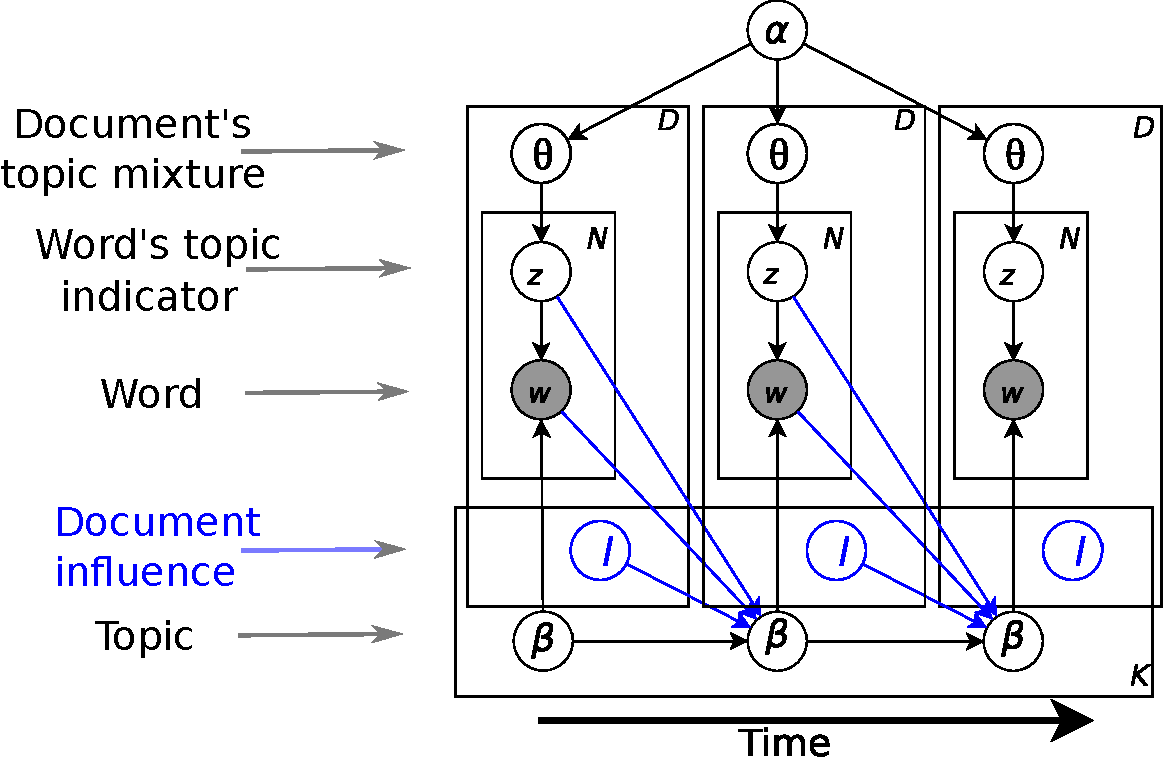
\includegraphics[width=1.0\linewidth]{../figures/docinf_gm.pdf}
  \caption{The Document Influence Model.  Edges between variables and
    non-adjacent topics have been dropped for clarity.}
 \label{fig:doc_influence_model}
  \vspace{-.1in}
\end{figure}

The influence of a document $d$ on each topic $k$ works as follows.
The more influential $d$ is on topic $k$ (i.e., the higher its weight
for this topic)--and the more its words are ''about'' topic $k$ in the
first place--the more it ``nudges'' this topic's natural parameters
$\beta_{t, k}$ in log space.  In LDA, and hence the DIM, the topic
assignment for word $n$ is given by the random variable $\z_n$; its
role is clarified below the generative model.

The full generative model at time $t$ is then:
\begin{packed_enum}
  \item For topic $k = 1, \ldots, K$: \label{gen:beta} \\
     Draw natural parameters \small $\beta_{t,k} | \beta_{t-1,k}, \z_{s<t}, l_{s<t} \sim$ \\
     \[
      \mathcal{N} \Bigg(\beta_{t-1,k}
      + \exp(-\beta_{t-1,k}) \circ \big( \sum_{i=0}^{t-1} r(t-1-i) g(t), \sigma^2 I \big) \Bigg),
      \]
\normalsize

      with $g(s)$ and $r(s)$ defined below.
  \item For each document $d \in D_t$:
      \begin{packed_enum}
	\item Generate all documents at time $t$ using LDA with topics
	  $\beta_{t}$.
	\item For topic $k = 1, \ldots, K$,  \label{gen:l}
	  draw document weight $\vec{l}_{d,k} \sim \mathcal{N}(\textbf{0}, \sigma_l^2 I)$,
      \end{packed_enum}

\end{packed_enum}
where above we have $g(s) := ([\z_{s}]_k \circ
 \W_{s}) l_{s,k}$,
with $\circ$ denoting the element-wise
 Hadamard product, $r(j)$ the
fraction of a document's influence after $j$ years, and $[z]_k$ the
indicator describing whether term $z$ is in
 topic $k$.  Specific
parameters are described in more detail in the following section.

In general, we do not want a document about the Earth's magnetic
fields to influence the use of words like ``magnet'' in the field of
medicine.  On the other hand, a document about fMRI should certainly
be allowed to influence the use of ``magnet'' in the field of
medicine.  In our model, this intuition is captured by the indicator
$[\z]_k$ in $g(s)$: documents not about medicine will tend to have
fewer words from the medicine topic, hence they will affect medicine
less.

In the model, $r(t)$, the \emph{influence envelope}, can be
interpreted as the fraction of a document's influence on the language
of some topic, $t$ epochs after it appears, with $r(i) > 0$ and $\sum r(i)
= 1$.  We assume here that $r(t)$ is fixed for all documents and all
time, although we plan to experiment with a more flexible model of $r$
in the future.  For the experiments and results described in this
paper, we have fixed $r(0) = 1$, although we are experimenting with
different envelope functions.

We believe that it is incorrect to add the words in each
document to the mean parameters, because this is like comparing apples
to oranges.  The coefficient $\exp(-\beta_{t-1})$ in the Markov step
handles this by mapping the documents, which are in ``word-space'', to
the space of natural parameters.  Recalling that $\beta$ gives the
natural parameters of a topic, and $\exp(\beta)$ gives the mean parameters
(relative word frequencies) of that topic, we see this result by
considering the contributions $I$ of documents for time $t$:
\begin{eqnarray}
& \exp(\beta_t) & = \exp(\beta_{t-1}) + I \nonumber \\
 \implies & \beta_t & = \beta_{t-1} + exp(-\beta_{t-1}) \log(1 + I) \nonumber \\
\end{eqnarray}

  When the influence $I$ is small,
$\beta_t \approx \beta_{t-1} + \exp(-\beta_{t-1}) I$, yielding the Markov step.
